\section{Simulation Analysis}

Using \textit{ngspice}, we began by analysing the circuit having obtained the following results for the voltage at the terminals of the envelope detector

\begin{figure}[htb!]
     \centering
     \begin{subfigure}[b]{0.45\textwidth}
         \centering
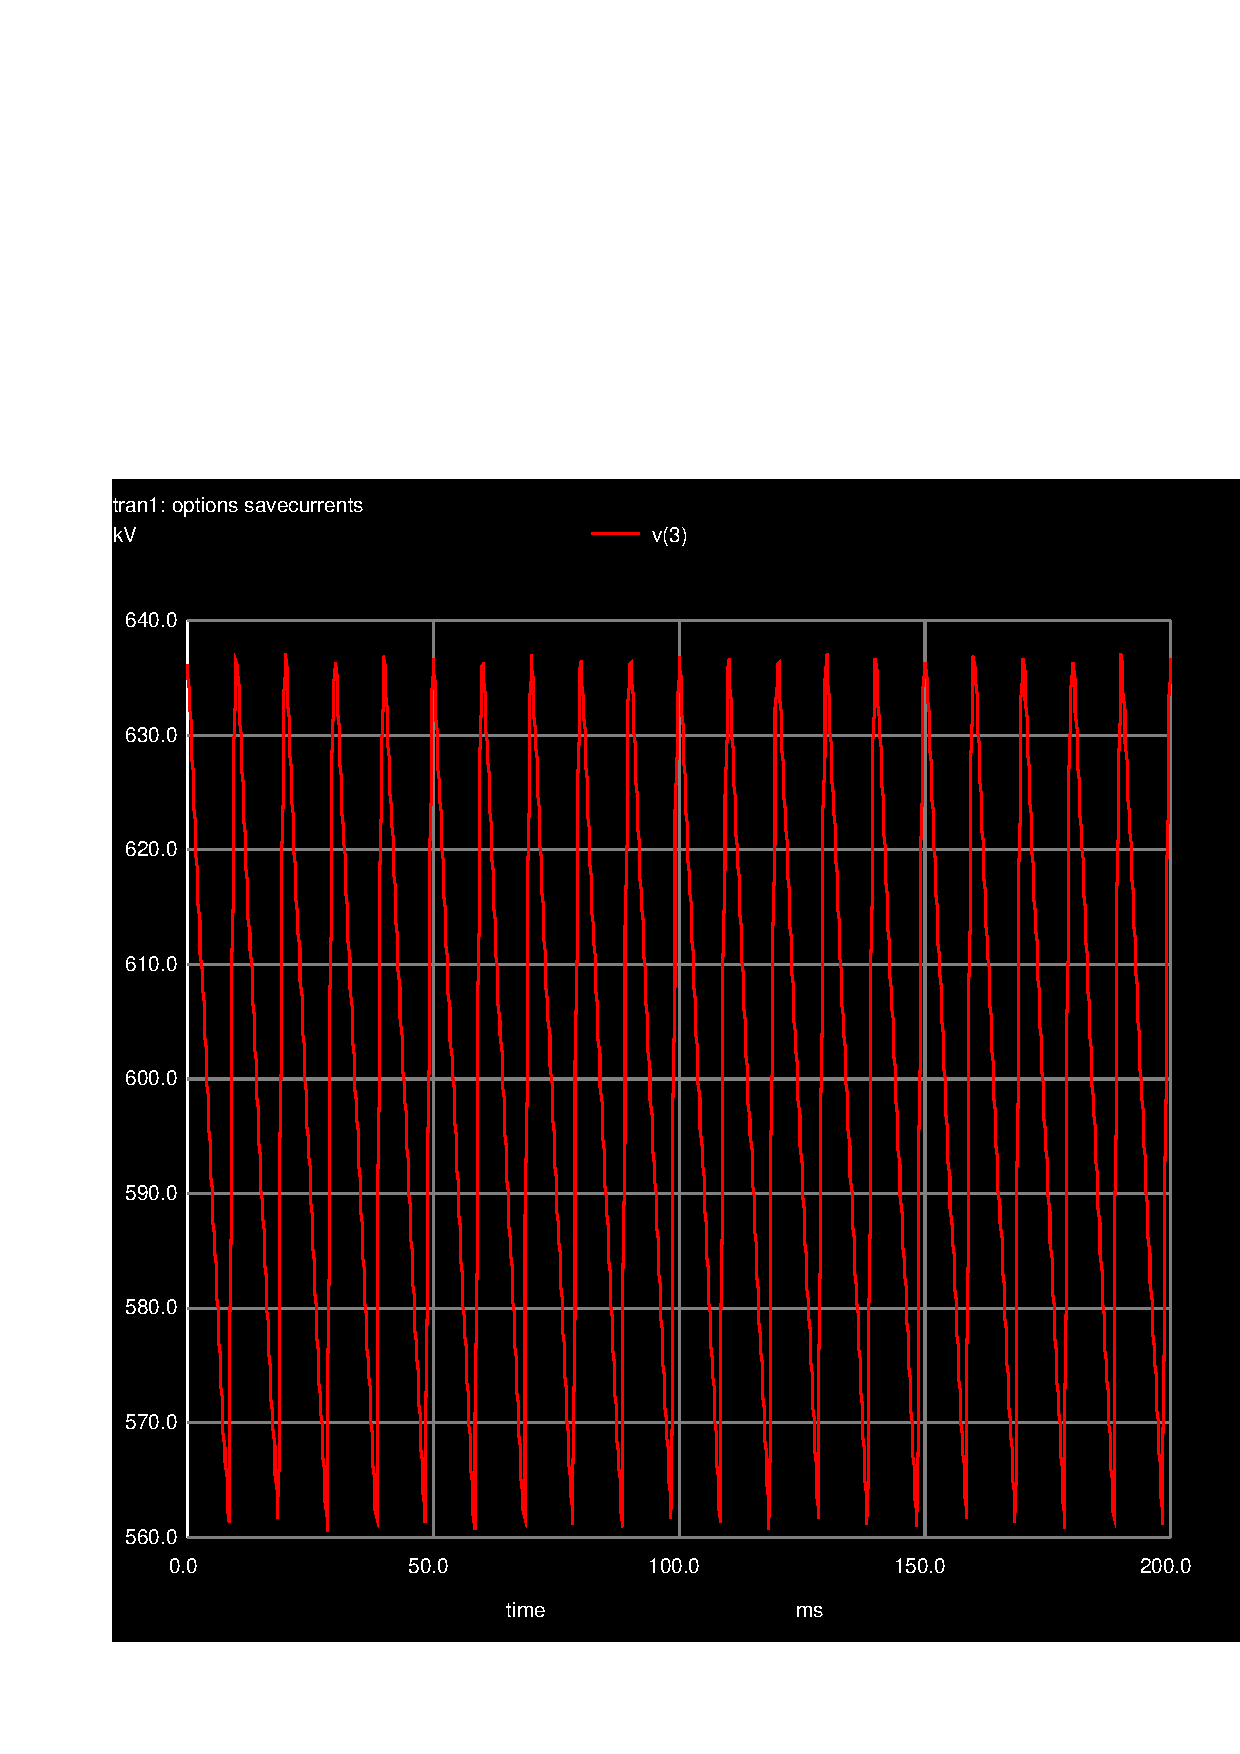
\includegraphics[width=\textwidth]{../sim/trans2.pdf}
\caption{Capacitor Voltage - Vertical axis in kV - \textit{ngspice}.}
\label{fig:TForcedP}
     \end{subfigure}
     \hfill
     \begin{subfigure}[b]{0.45\textwidth}
         \centering
\includegraphics[width=\textwidth]{../mat/venvlope.png}
\caption{Capacitor Voltage - Veritcal axis in V - \textit{Octave}}
\label{fig:TForcedP}
     \end{subfigure}
     \hfill
     \caption{Envelope circuit output}
     \label{fig: graphsEnv}
\end{figure}


At this point the voltage is already semi-stable, having a small ripple effect, which was corrected with the voltage regulator circuit. It should also be noted that, while the overall shape and frequecy of oscilation is the same, there is a significant difference in the amplitude of the signal which radicates from the ideal diode approximation used in the theoretical analysis.

\begin{figure}[htb!]
     \centering
     \begin{subfigure}[b]{0.45\textwidth}
         \centering
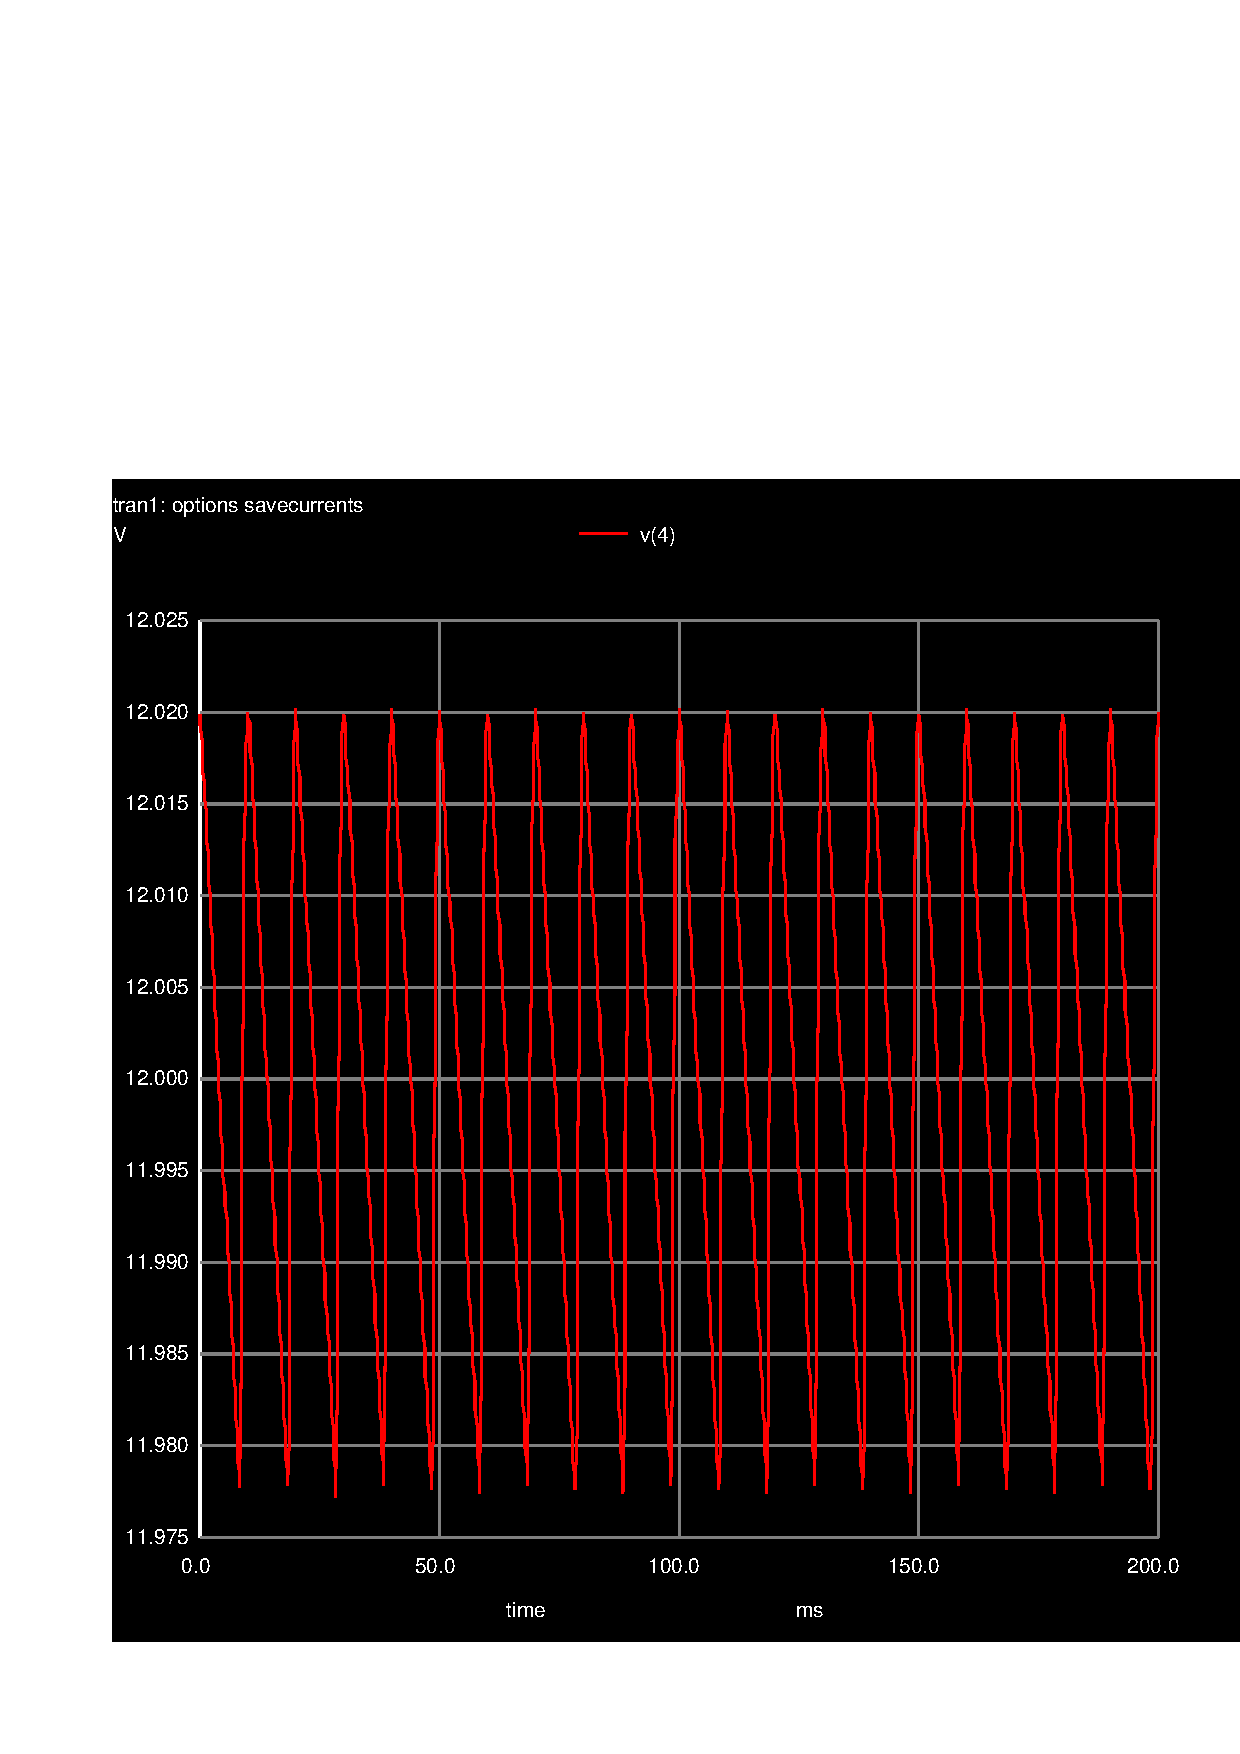
\includegraphics[width=\textwidth]{../sim/trans.pdf}
\caption{Output Voltage - Vertical axis in V - \textit{ngspice}.}
\label{fig:TForcedP}
     \end{subfigure}
     \hfill
     \begin{subfigure}[b]{0.45\textwidth}
         \centering
\includegraphics[width=\textwidth]{../mat/OutputV.png}
\caption{Output Voltage - Veritcal axis in V - \textit{Octave}}
\label{fig:TForcedP}
     \end{subfigure}
     \hfill
     \caption{Circuit output}
     \label{fig: graphsEnv}
\end{figure}


The output voltage is much more stable, having a signal with far less amplitude. Moreover, the diodes also diminish the overall value of the voltage, lowering the average to approximatly the desired value of 12V.

\begin{figure}[htb!]
     \centering
     \begin{subfigure}[b]{0.45\textwidth}
         \centering
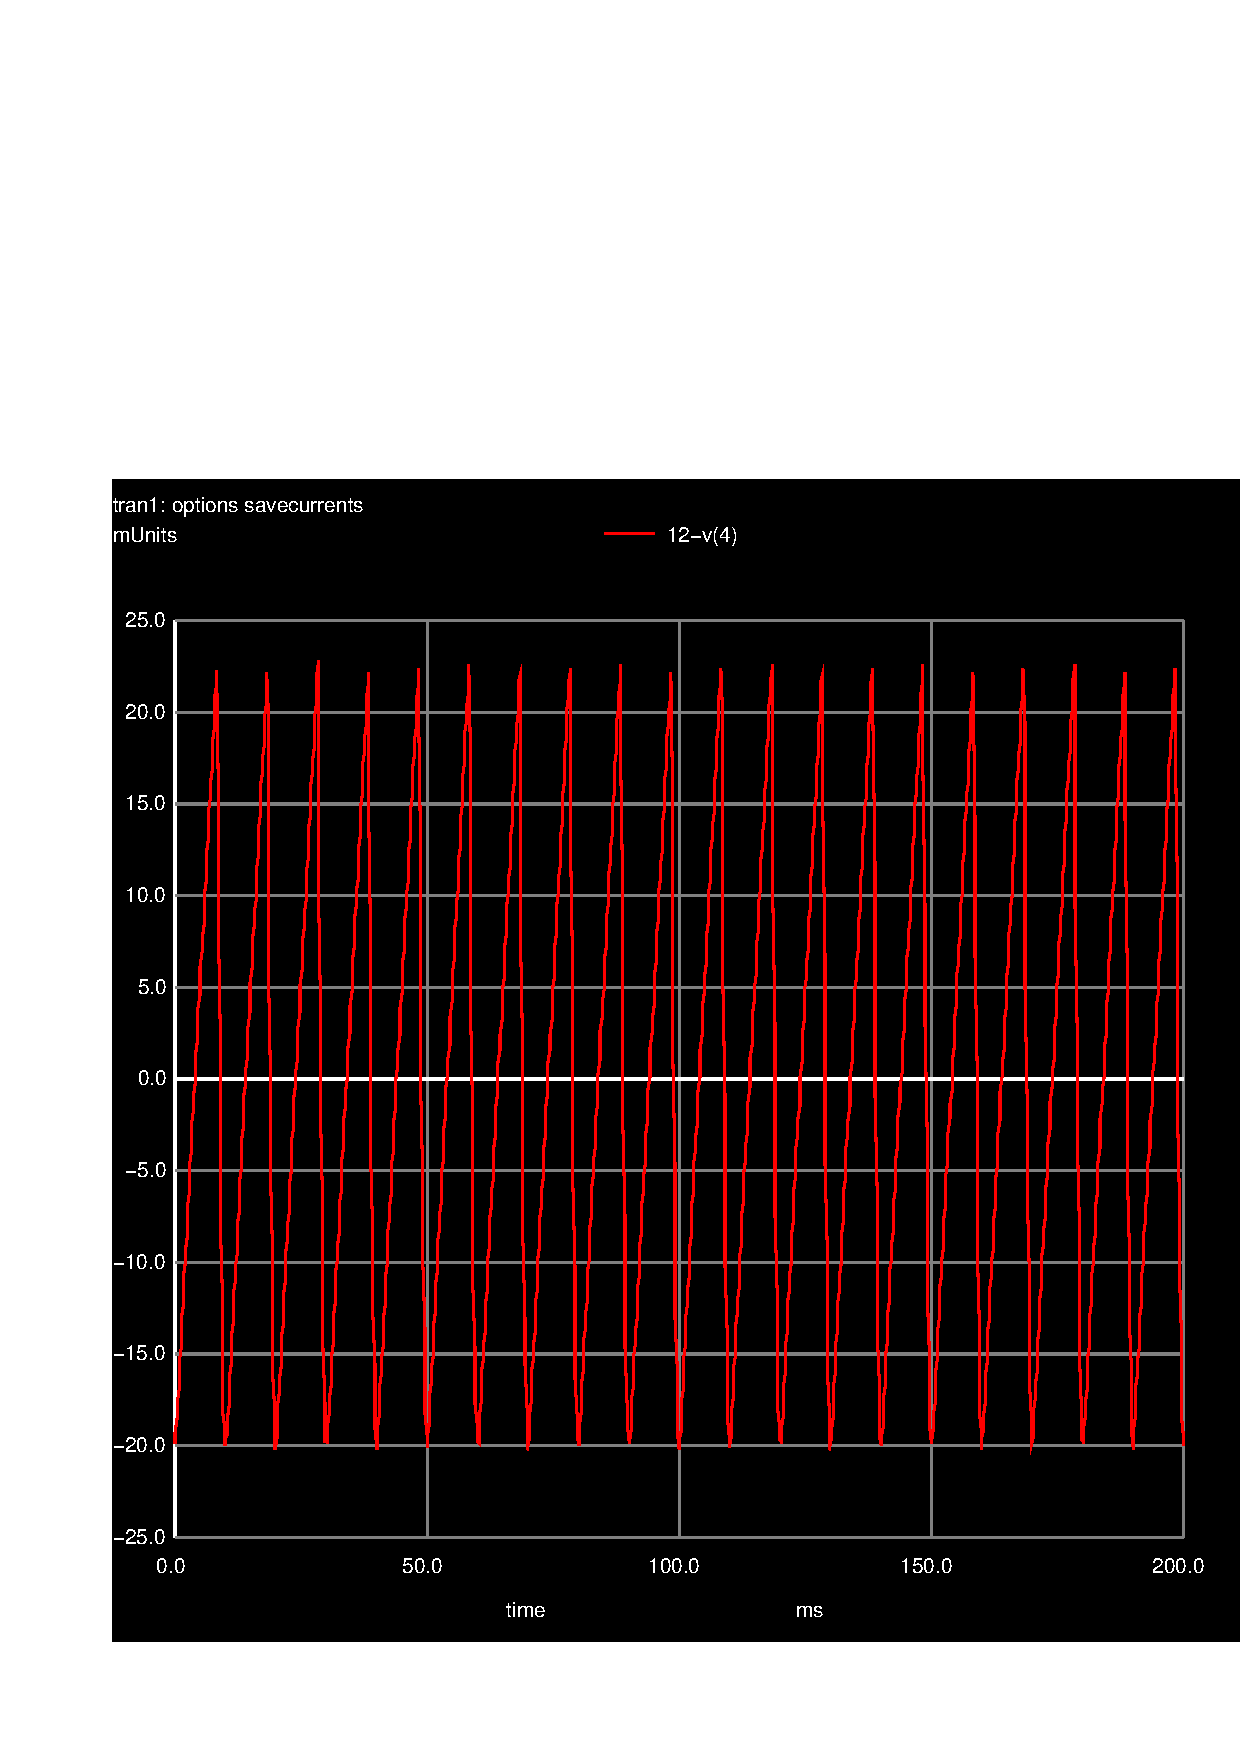
\includegraphics[width=\textwidth]{../sim/trans4.pdf}
\caption{Output Voltage-12V - Vertical axis in mV - \textit{ngspice}.}
\label{fig:TForcedP}
     \end{subfigure}
     \hfill
     \begin{subfigure}[b]{0.45\textwidth}
         \centering
\includegraphics[width=\textwidth]{../mat/Level.png}
\caption{Output Voltage-12V - Veritcal axis in V - \textit{Octave}}
\label{fig:TForcedP}
     \end{subfigure}
     \hfill
     \caption{Output voltage-12V}
     \label{fig: graphsEnv}
\end{figure}


Once again, there are obvious differences from the theoretical analysis: the predicted voltage is much closer to 11V and the amplitude of the oscilation approximatly halved compared to their \textit{ngspice} counterparts. Nontheless, this divergence can be inputed to \textit{ngspice's} much more complex diode model and to the theoretical approximations made in the envelope detector analysis.
Therefore, we chose to calculated the Merit figure for the transformer using the simulation results, having thus obtained


\begin{table}[h]
  \centering
  \begin{tabular}{|l|r|}
    \hline
    f & 1.004690e+03\\ \hline
gain & 3.652900e+01\\ \hline
z & 1.519501e+03\\ \hline

  \end{tabular}
  \caption{Output voltage DC-Level and Ripple (Maximum - Minimum)}
  \label{tab:op1}
\end{table}
